%! Author = Franciszek Świderski
%! Date = 12/10/2024

% Preamble
\documentclass{report}

\usepackage{graphicx}

\usepackage{float}
% Packages
\usepackage{amsmath}

% Document
\begin{document}
    \begin{titlepage}
        \centering

        {\Huge Data warehousing of European parliament voting data and Unsupervised Learning\\}

        \vspace{1cm}

        {By \textbf{Franciszek Świderski}\\}

        \vspace{1cm}

        {B. Sc. International Politics and Government, Bocconi University\\}
        \vspace{1cm}
        {Under the supervision of\\}
        \vspace{1cm}

        {\textbf{Omiros Papaspilioupoulos}\\}

        \vspace{1cm}
        {Full Proffesor at Department of Decision Sciences, Bocconi University\\}
        \vspace{1cm}

        {For Institute for European Policymaking at Bocconi University\\}
        \vspace{1cm}
        {October 2024\\}

        \vspace{5cm} % Add some space between the title and author information


    \end{titlepage}

    \begin{abstract}
        Abstract goes here
    \end{abstract}

    \tableofcontents


    \chapter{Introduction}
        This is an introduction to the work, I do some intorducting


        \section{Dataset Structure and Initial Challenges}

            The dataset comprises three primary components:


            \begin{itemize}
                \item MepInfo: This dataset contains information on Members of the European Parliament (MEPs).
                \item Votes: This dataset records the votes cast by MEPs on specific pieces of legislation.
                \item Votings: This dataset describes the legislative items that were voted upon.
            \end{itemize}
            \begin{figure}[htb]
                \centering
                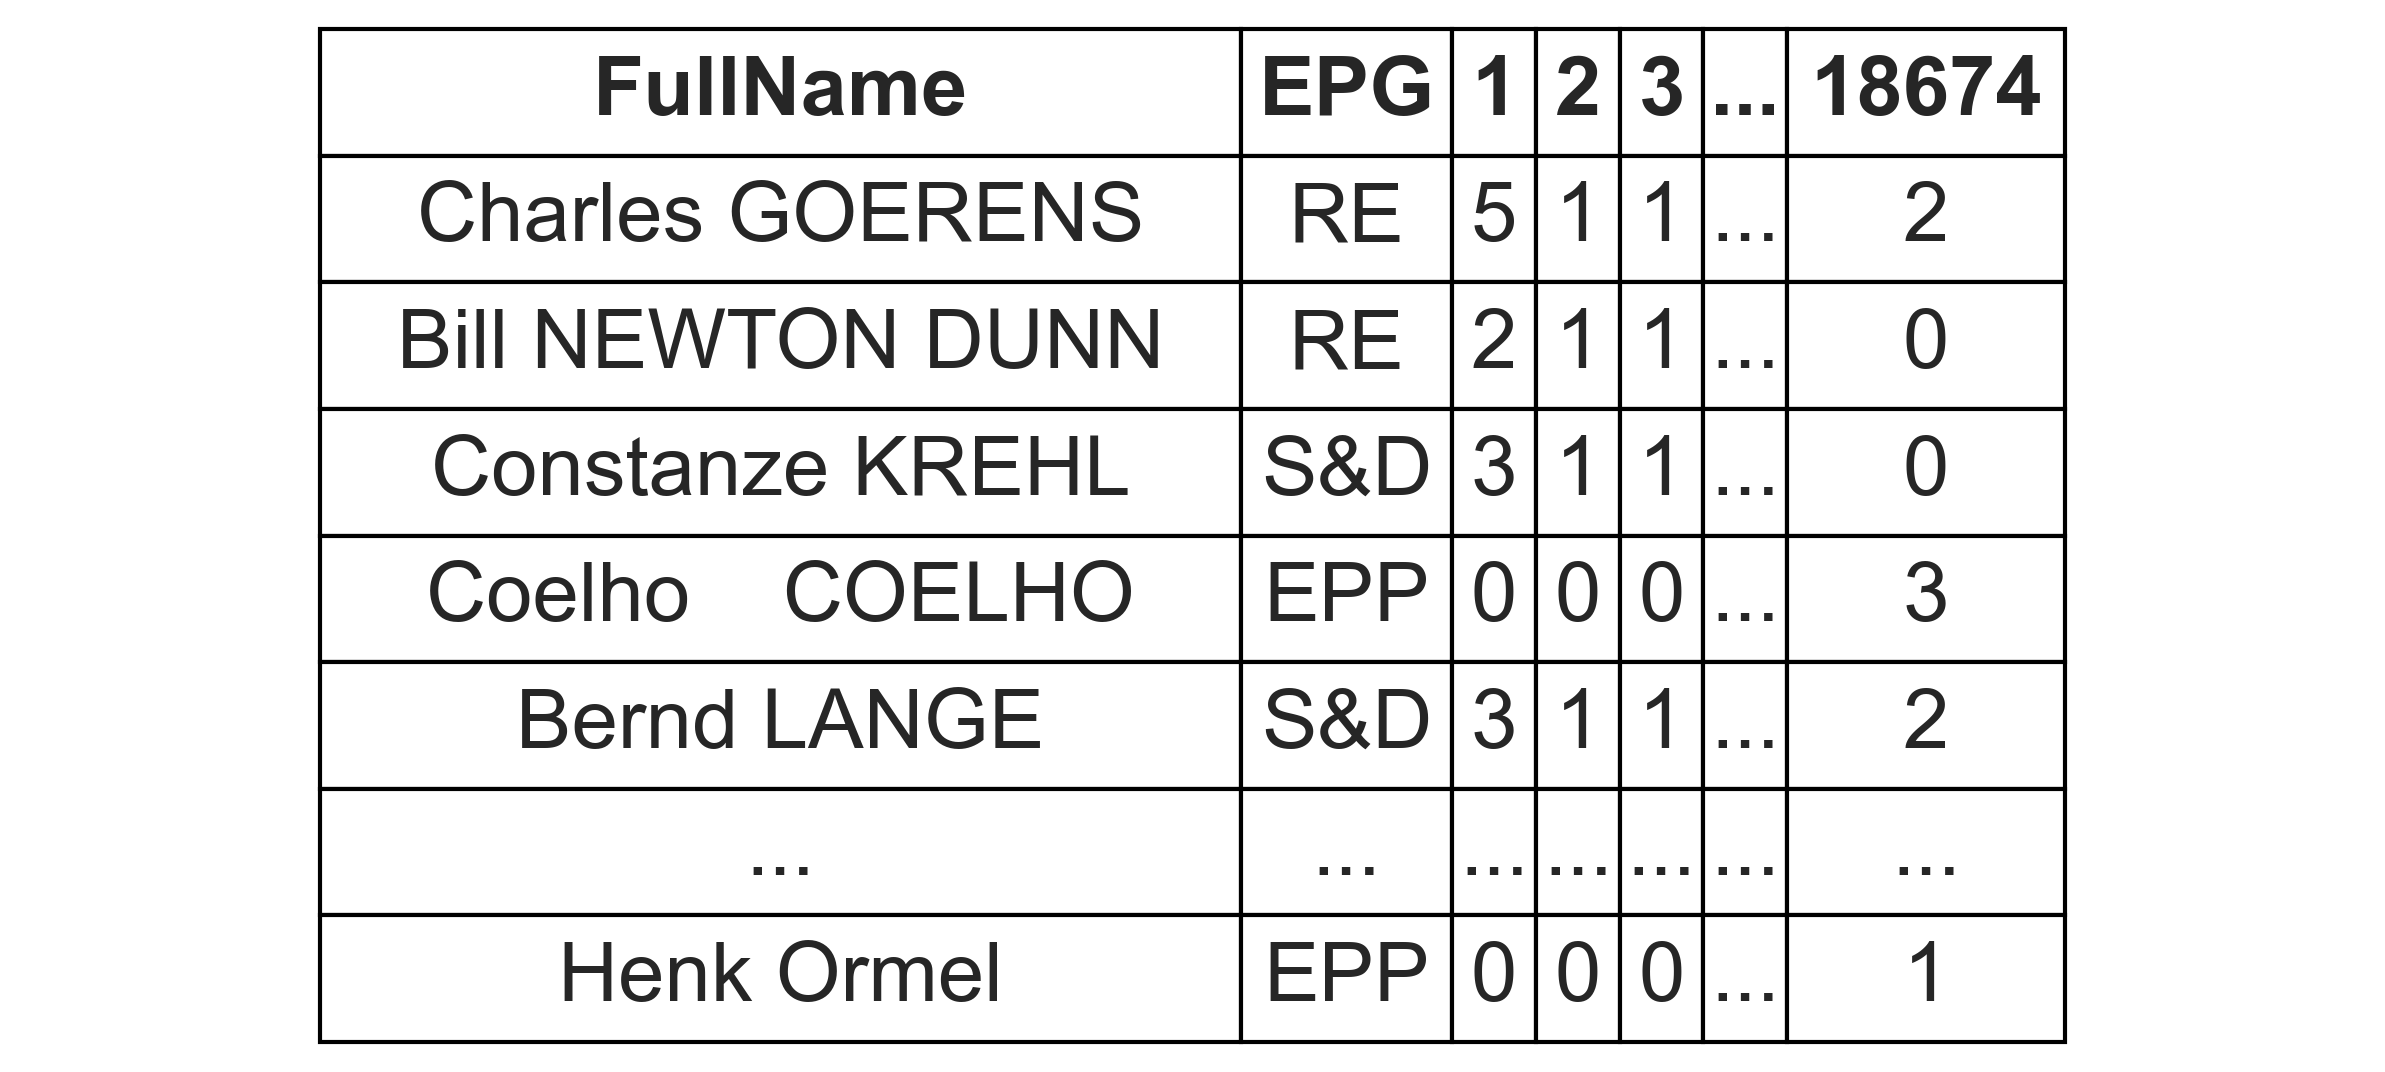
\includegraphics[width=1\textwidth]{Graphs/short_table9.png}
                \caption{Data from European Parliament 9 formatted for roll-call scaling}
                \label{fig:Structure table}
            \end{figure}

            The Votes dataset alone includes approximately 42,800 roll-calls, with 800-900 MEPs participating in each
            legislature, resulting in an estimated 40 million data points.
            \begin{figure}[htb]
                \centering
                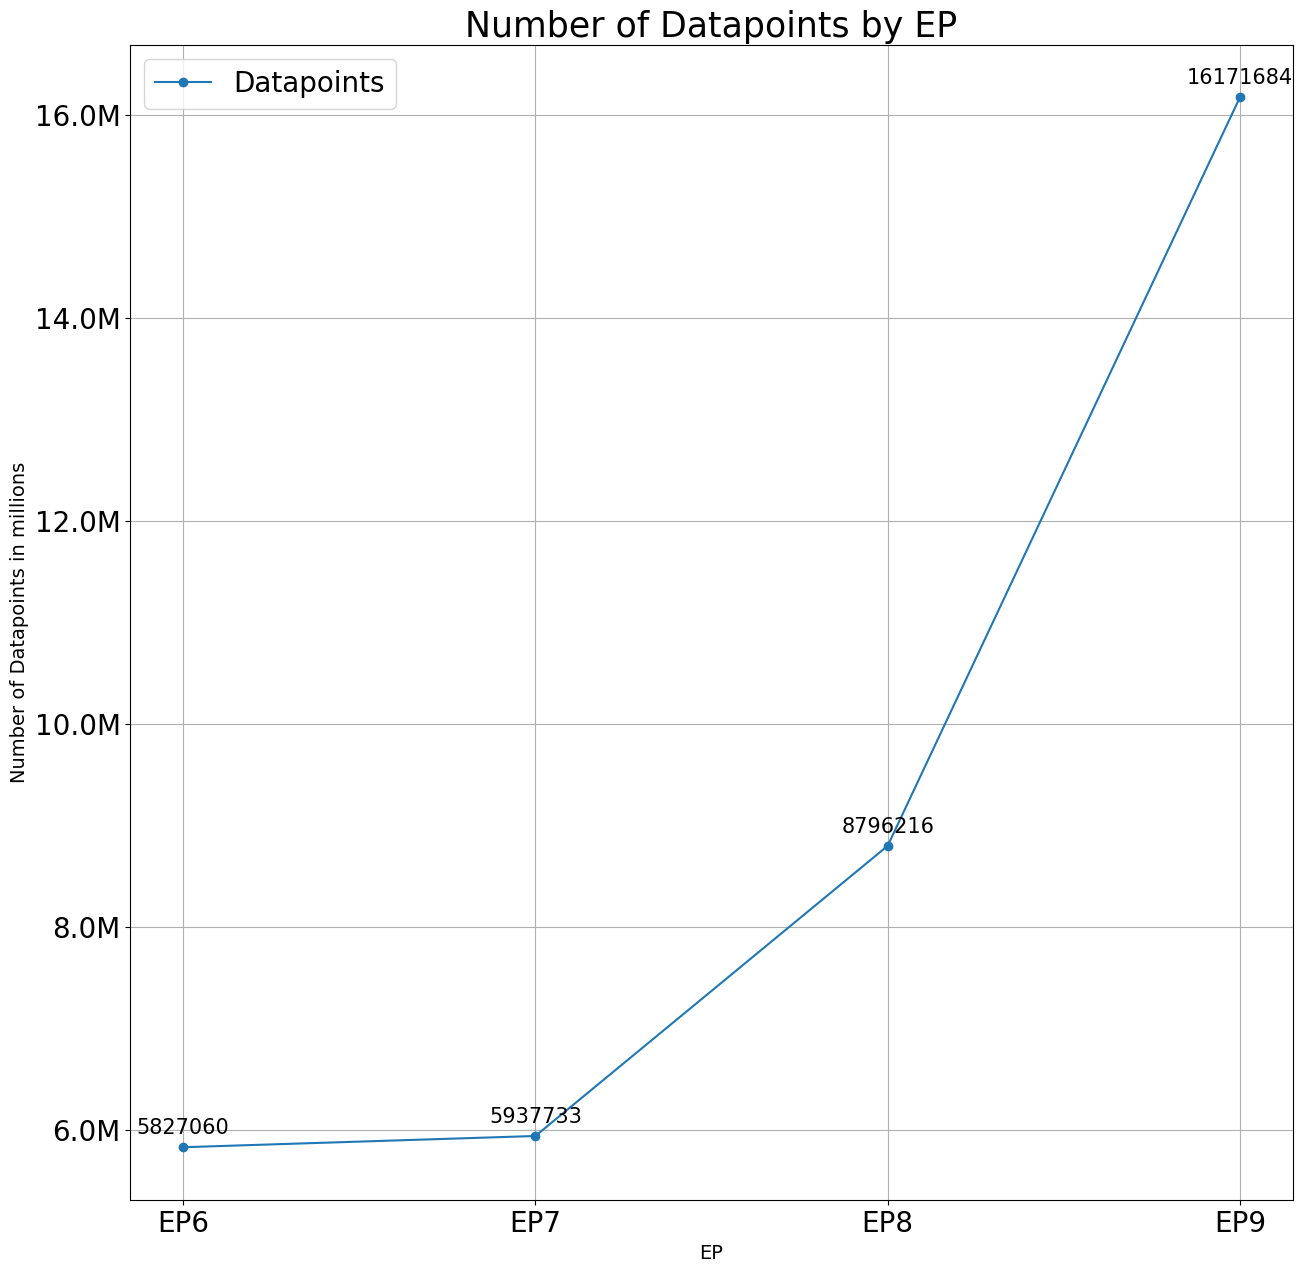
\includegraphics[width=0.8\textwidth]{Graphs/Datapoints.png}
                \caption{Number of datapoints by European Parliament (EP)}
                \label{fig:Datapoint graph}
            \end{figure}

            The size of the dataset makes for a serious practical challenge in terms of storage and processing, not to
            mention the problems with formatting and integrity of the dataset. Upon initial examination, several issues
            with the
            legacy data became apparent:

            \begin{itemize}
                \item
                Missing Variables: The MepInfo dataset lacked several critical variables, including gender and age.
                \item
                Inconsistencies and Missing Observations: Some variables such as Party affiliation and European
                Parliament Group
                (EPG) affiliation were either inconsistent or incomplete.
                \item
                Non-Standard MEP IDs in EP7: MEP IDs in the 7th Parliament did not conform to the standard European
                Parliament
                API format. Instead of unique identifiers, incrementing integers were used.
                \item
                Naming Conventions: MEP names and surnames were not consistent with those in the European
                Parliament API.
                \item
                Incorrect and Inconsistent Encoding of Missing Data: Missing data was inconsistently encoded, with
                symbols like
                - or . being used in place of null values.
                \item
                Inconsistent Datetime Formatting: Datetime values were formatted inconsistently across the dataset,
                making them
                difficult to import and process.
                \item
                Non-Standard Encoding of Binary Categorical Variables: For example, the binary categorical variable "
                Vote,"
                which indicates whether a vote passed or not, was encoded as + and - instead of the standard 1/0 used
                elsewhere
                in the dataset.
            \end{itemize}
            Additionally, the dataset was stored in a long format tailored to the specific analytical requirements of
            the
            original VoteWatch team. While this structure was suited to their immediate needs, it posed challenges for
            long-term
            usability, warehousing, and broader analytical purposes.


    \chapter{Data Cleaning Process}


        \section{Supplementing and Correcting the MepInfo Dataset}


            The initial challenge involved supplementing and correcting the MepInfo dataset to fill in missing variables
            and
            rectify inconsistencies. The European Parliament's API played a crucial role in this process. An API
            (Application
            Programming Interface) is a set of defined rules and protocols that allows one software application to
            interact with
            another. In the context of scraping data, an API serves as an intermediary that lets users request and
            retrieve
            specific data from a website or service in a structured format, typically JSON or XML, without the need to
            manually
            scrape the HTML content of a webpage.
            Using an API for data scraping is often more efficient and reliable than traditional web scraping, as it
            provides
            direct access to the desired data, reducing the risk of encountering issues like changes in webpage
            structure or
            content restrictions. This API provides endpoints, such as `/meps`, which return JSON data containing basic
            MEP
            information, including a unique identifier (MepId). By utilizing this API, we were able to standardize the
            names and
            identifiers of MEPs across most legislatures by joining the tables by MepId.

            However, the 7th Parliament (EP7) presented a unique challenge. The MEP IDs in this legislature were not
            unique and
            were instead represented by incrementing integers. To address this issue, we employed the `fuzzywuzzy`
            Python
            package, which uses the Levenshtein distance algorithm to calculate the similarity between strings. This
            allowed for
            making an approximate match of full names from the original dataset to the `sortLabel` field in the API
            data,
            providing the correct MEP IDs. Manual verification and correction of edge cases were necessary to ensure
            accuracy.

            Despite these efforts, some data remained incomplete, particularly regarding MEPs who changed parties or
            EPGs during
            their tenure, as well as demographic data such as gender and birth dates. These gaps required further manual
            supplementation, which is discussed in detail in the Automation section.


        \section{Addressing Inconsistencies in the Votings Dataset}

            The Votings dataset required significant work to address encoding inconsistencies and improperly formatted
            datetime
            values. The first issue was relatively easy to reconcile using renaming dictionaries to replace inconsistent
            encodings in some variables.

            However, the latter issue proved particularly problematic due to the original data being gathered in Excel.
            Manual
            formatting likely led to inconsistent datetime values formatting. To standardize the format, manual
            correction of
            the dates was necessary before applying the Pandas `to datetime` function.

            This step ensured that the datetime values were correctly parsed and made the data suitable for further
            analysis.
            Once the initial cleaning was complete, a new challenge arose. In 2022, the original VoteWatch team altered
            their
            data gathering methodology. Consequently, data from Parliament 9, covering the period until 2022, was
            consistent
            with earlier practices. However, data collected from 2022 to March 2024 exhibited several discrepancies. The
            order
            of VoteIds had changed, some columns particularly those in the Votings dataset were missing, and special
            characters
            were corrupted due to encoding issues.
            To resolve these issues, we employed a multi-step approach. First, we used a dictionary to replace the
            corrupted
            characters systematically. Next, we reverse-engineered the missing Votings columns (such as finalVote, a
            binary
            variable of whether a vote is a last one in a section) from the available data. Despite the complexity of
            these
            tasks, they were necessary to restore the integrity and consistency of the dataset, ensuring that it could
            be
            seamlessly integrated with the existing data from earlier legislative periods.


        \section{Data Restructuring for Long-Term Usability}

            With the Votes and MepInfo datasets cleaned and supplemented, the next step was to restructure the data into
            a
            format suitable for long-term storage, analysis, and future updates. The data was initially stored in a long
            format,
            where each row represented an observation, and columns represented variables. To facilitate analysis, we
            separated
            the MepInfo and Votes datasets into distinct tables:
            \begin{itemize}
                \item
                MepInfo table contained all variables describing the MEPs, with `MepId` serving as the primary key.
                \item
                The Votes table used a composite primary key consisting of `MepId` and `VoteId`, a unique identifier for
                each
                voting event. This table also included a column encoding the MEPs' votes.
            \end{itemize}

            These tables were linked by primary keys, allowing for efficient querying and data retrieval. For example,
            using the
            `MepId`, one could easily retrieve all votes cast by a particular MEP, and by further referencing the
            `VoteId`,
            additional context from the Votings table could be added.

            To support the development of the European Parliament Vote Monitor website, the voting data was additionally
            exported in `.csv` format, organized by month and year. This format was chosen to optimize data storage and
            accessibility, ensuring that the data could be easily updated and queried. Additionally, for specialized
            analytical
            purposes, the Votes data was also retained in its original matrix format, now enhanced with the newly
            cleaned and
            supplemented variables.


    \chapter{Automation of Data Gathering}


        \section{Overview of the European Parliament API}

            With the historical data cleaned and restructured, the next phase of the project focused on automating the
            future
            data gathering process. Consistency and reliability were paramount in this process. The previous VoteWatch
            team
            relied on scraping XML files from the human-readable official minutes on the European Parliament's website,
            coupled
            with downloading MepInfo from the API. This approach was fraught with challenges, including the potential
            for
            inconsistencies in the scraped data, lack of unique identifiers, and the inherent unreliability of scraping
            human-readable content.

            To address these issues, we transitioned to using the European Parliament's open API, which provides direct
            access
            to structured data in a reliable and consistent manner. The API is publicly accessible, meaning no API key
            is
            required, and it allows users to specify parameters in the URI to retrieve data from various endpoints.


        \section{MepInfo Data Collection Automation}
            The `/meps` endpoint of the API, which provides a list of MEPs along with their unique identifiers, was the
            starting
            point for automating the MepInfo data collection. However, the data returned by this endpoint was not
            exhaustive. To
            gather more detailed information such as MEPs' gender, age, and political affiliations additional API calls
            were
            required to other endpoints within the `meps` group.

            For example, to retrieve data on MEPs' party memberships and affiliations with European Political Groups
            (EPGs) and
            National Parties, separate API calls were made specyfing the MepId . The resulting data was then filtered
            and joined
            with the MepInfo dataset to create a comprehensive record of each MEP s political affiliations and
            demographic
            information.

            One key challenge in this process was optimizing the API calls to minimize the load on the server. Each MEP
            required
            an individual API call to gather detailed data, which could result in approximately 850 GET requests per
            scraping
            session. To mitigate this, the metadata was included in the same call to avoid the need for additional
            requests.

            Another consideration was the use of non-human-readable IDs for certain values, such as the organization
            field,
            which required further API calls to retrieve the corresponding labels from the `corporate-bodies` endpoint.
            For
            example org/1537 was an identifier for GUE/NGL EU Political Group. These labels were essential for
            understanding the
            data and were subsequently joined with the MEPs' political affiliation data.


        \section{Votings Data Collection Automation}

            The `meetings` endpoint of the API was utilized to automate the collection of data on plenary sessions and
            the
            decisions made during these sessions. An initial API call returned a list of all plenary sessions that took
            place in
            a given year. This list was then filtered by month to identify the specific sessions relevant to the current
            data
            collection period.

            For each identified session, further API calls were made to retrieve detailed voting data, such as the votes
            cast by
            each individual member and all of the supplementary data that was previously found in the Votings database.
            This
            data was then merged with the previously gathered MepInfo and Votes data, ensuring that all relevant
            information was
            captured and linked across the collection.

            In order to automatically gather the data in the future, working with a Bocconi IT Department team, we
            created a
            cloud-based solution that is deployed and triggers every month, gathering and exporting the data to the .csv
            format,
            as well as to a relational SQL database.


    \chapter{Ideal Points Estimation - Overview of Current Methods}
        One of the most prominent uses of voting data in political science research is estimating ideal points of
        legislators on the ideological plane. The early revolutional work of Poole and Rosenthal (1985) set the
        precedent for using those types of algorithms - specifically NOMINATE - Nominal Three Step Estimation on
        larger datasets than previously possible. Ever since, ideal points estimation was developed more and more,
        with improved versions of the original algorithm (such as D-NOMINATE, and later W-NOMINATE), to extending
        its implementation beyond the original usecase (scaling the US parliament), analysing the European
        Parliament and various national parliaments. The European parliament specifically has had a great deal of
        coverage using the WNOMINATE method, which has been the standard for the past 20 years.


        \section{WNOMINATE}

            \subsection{Algorithm}

                W-NOMINATE (Weighted NOMINATE) - an improved version of NOMINATE, used for estimating legislator's
                ideal points relying on their roll-call voting records. The underlying model of NOMINATE, and by
                extention, W-NOMINATE is a spatial voting model, where legislators and the policies are represented
                in a multidimensional space. In this implementation, a legislator has an ideal point in this space,
                that represents their ideology and policy preference, and each vote is a set of two alternative
                points - one when the policy is implemented (the vote passes), and another when the policy is
                rejected (the vote fails). W-NOMINATE assumes that legislators vote for an outcome that is closest
                to their ideal point, with some random error to account for unpredictability.

                The utility a legislator derives from a vote is modeled as a function of the Euclidean distance between
                their ideal point and the vote outcome locations. Legislators aim to maximize their utility by voting
                for the outcome that minimizes the distance to their ideal point. The model uses the following utility
                function:

                \[
                    U_{ijy} = \beta \exp \left[ -\sum_{k=1}^{s} w_k^2 (x_{ik} - z_{jy})^2 / 2 \right]
                \]

                where:
                \begin{itemize}
                    \item \( x_{ik} \) is the ideal point of legislator \(i\) on dimension \(k\),
                    \item \( z_{jy} \) is the position of the "yea" outcome for vote \(j\),
                    \item \( \beta \) controls the ratio of deterministic to stochastic utility,
                    \item \( w_k \) is a weight for each dimension.
                \end{itemize}

                The likelihood of voting "yea" is determined by comparing the utilities of the two possible outcomes (
                yea or nay). W-NOMINATE estimates the legislators' ideal points and vote outcome locations iteratively,
                using maximum likelihood estimation. The process continues until the estimates stabilize and a
                convergence threshold is met. Typically, one or two dimensions are used in most applications, with the
                first dimension often capturing the left-right ideological spectrum.

            \subsection{Initialization}
                The initialization of W-NOMINATE requires setting initial values for the legislators' ideal points and
                vote outcome positions. These are assigned by estimating the positions of
                the legislators by calculating an agreement matrix. It is calculated by assigning values (in this
                case, they were most likely chosen heuristically) to each vote, Yea is 1, Nay is 6 and Missing (
                abstentions, etc. ) are 9. Then the program iterates over each vote in each pair of legislators,
                calculating the average distances between their votes and storing it in a square matrix. Then the
                eigenvectors of this matrix are used as starting points for the algorithm to iterate


                The key parameter \( \beta \) is usually set to an initial value of 15, indicating that the
                deterministic component of utility
                strongly outweighs the stochastic component.

                Additionally, a "lop" threshold is set to determine which votes are included in the analysis.
                This threshold excludes votes where too many legislators vote in the same way, as these votes
                provide little information about ideological differences. The default value is 0.025,
                meaning that votes where fewer than 2.5\% of legislators voted in the minority are excluded.

            \subsection{Implementation}
                W-NOMINATE is implemented in the \texttt{wnominate} package for \texttt{R}
                , which builds upon earlier Fortran-based implementations. The package simplifies data input and
                provides tools for estimating ideal points and visualizing results. Roll-call data is typically
                stored in a \texttt{rollcall} object from the \texttt{pscl}
                package. The iterative maximum likelihood estimation process continues until the ideal points
                and vote outcomes converge, defined as a correlation of 0.99 between successive iterations.

                The \texttt{wnominate}
                package also includes an option for bootstrapping to estimate standard errors. Users can specify
                the number of bootstrap trials, with the default being no bootstrapping. Visualizations, such as
                plots of ideal points and vote outcome locations, are also provided to facilitate interpretation
                of the results.

                While the package has been the standard in political sciences for the past 20 years, the software
                implementation has its' limitations. Lack of multi-threading support does not take advantage of the
                computing power of new machines effectively and the algorithm is prohibitively slow when working
                with larger datasets, such as the European Parliament 9 votes.


        \section{emIRT}

            \subsection{Algorithm}
                In order to circumvent the limitations of the traditional methods Imai, Lo, and Olmsted (2016) developed
                a
                new algorithm, emIRT - it is particularly efficient in estimating the ideal points in large datasets -
                where
                traditional methods, such as Markov Chain Monte Carlo
                (MCMC) or the NOMINATE procedure , are computationally expensive. emIRT uses the
                Expectation-Maximization (EM) framework, which is faster and more scalable.

                At the core of emIRT is an item response theory (IRT) model, where legislators' votes are treated as
                indicators of latent ideological preferences (ideal points). The algorithm estimates ideal points by
                iterating between two steps:
                \begin{itemize}
                    \item \textbf{E-step}
                    : The algorithm computes the expected value of the latent variables (the legislators' underlying
                    voting propensities) given the current estimates of the ideal points and vote parameters.
                    \item \textbf{M-step}
                    : It updates the estimates of the ideal points and discrimination parameters by maximizing the
                    expected log-likelihood calculated in the E-step.
                \end{itemize}
                The process repeats until convergence. Unlike MCMC, EM is deterministic, converging faster and without
                the need for sampling. emIRT can handle binary, ordinal, and continuous voting data, making it highly
                flexible. It can also extend to dynamic and hierarchical models, where ideal points change over
                time or across groups.

            \subsection{Initialization}
                emIRT requires random initialization for the ideal points and the discrimination
                parameters.

            \subsection{Implementation}
                The emIRT algorithm is implemented in the \texttt{emIRT} package for \texttt{R}
                , which is designed to handle large-scale datasets efficiently. The package includes several
                models, including:
                \begin{itemize}
                    \item \textbf{Binary IRT models}: For binary voting data,
                    \item \textbf{Ordinal IRT models}: For ordinal voting data,
                    \item \textbf{Dynamic IRT models}: For time-varying ideal points,
                    \item \textbf{Hierarchical IRT models}: For nested data structures.
                \end{itemize}

                The algorithm performs Expectation-Maximization to estimate the ideal points and vote parameters. It can
                also estimate standard errors using a parametric bootstrap, simulating datasets based on the estimated
                model and then re-estimating the parameters to compute uncertainty. The package handles missing data in
                roll-call voting datasets by treating abstentions as latent variables to be predicted from the observed
                data. This ensures that the ideal points reflect complete voting behavior.


    \chapter{Ideal points estimation - using the software (very much working name)}
        Having understood, cleaned and restructured the data, the natural next step was using it for research.
        However, before going further, we needed to verify the integrity of the data - whether the cleaning process
        impacted the dataset in a meaningful way that would distort the results. In order to achieve this, we set
        out to recreate the workflow that Hix and Noury (all the years) used to reproduce their results. If the
        results were comparable to theirs, that would mean the dataset is functionally the same, as well as allowing
        us to use the workflow for further research.


        \section{Reproduction of results in Hix & Noury 2009}
            The first step in the process of veryfing the integrity of the data was to establish a reference point of
            comparison. The data we are working with spans from EP6 to EP9. The publications where Hix & Noury
            explicitly state the use of NOMINATE to create the two-dimensional representations of ideology in the
            European Parliament cover the range of EP1 to EP6 (later publications, like Hix, Noury & Rolland (2018) do
            not
            explicitly state the method of roll-call scaling and the results point to use of another method). This meant
            that the workflow reproduction is feasible in EP6, so we decided to pursue this direction.

            \subsection{Workflow reproduction}
                Having chosen the specific datset to produce the results from, we begun investigating the
                        \texttt{wnominate}
                package for \texttt{R}
                        described in Chapter 4. The documentation of the package in CRAN (The Comprehensive R
                        Archive Network - the package manager for R) lays out the steps for scaling an arbitrary (e.g.
                        not from the US
                        parliament) dataset of roll-call votes. The first step is importing the dataset and converting
                        it to a
                \texttt{rollcall} object from the \texttt{pscl}
                        package. This object store the votes and decsriptive data about
                        legistators in accordance with the \texttt{wnominate}
                        requirements. It recodes the votes to only contain 4
                        categories - 'yea' , 'nay' , 'missing' and 'not in legislature'. As previously mentioned, the
                        votes are stored
                        in the long format matrix - specific votes are columns, and each row is a legislator. From this
                        point on, the
                        only step required to initialize the algorithm is choosing the parameters \( \beta \)
                        and 'lop', as well as the '
                        polarity' of the dataset.

                \begin{figure}[H]
                    \centering
                    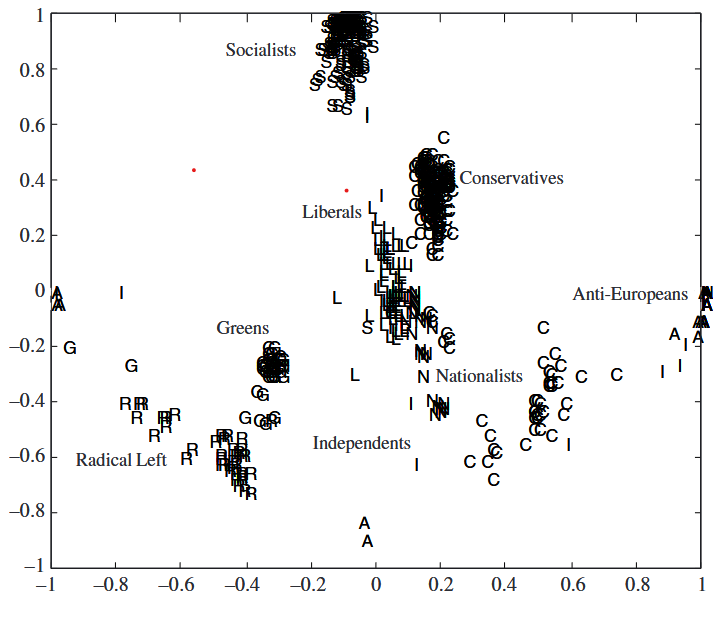
\includegraphics[width=1\textwidth]{Graphs/Screenshot 2024-06-09 220607.png}
                    \caption{Ideal points estimates from Hix&Noury (2009)}
                    \label{fig:WNOMINATEHIX6}
                \end{figure}


                As we do not have access to the code used for the analysis done by Hix and Noury, we have to make
                assumptions as
                to the parameters that they chose. \( \beta \)
                        and 'lop' have default values, heuristically assigned by the
                        creators of the software, and researchers usually do not change those. The issue arises with the
                        "polarity"
                        parameter. It requires the researcher using the package to choose a 'conservative' MP and the
                        algorithm will
                        center the result around his final position - so if the 'polarity' is chosen as (10,10), as it
                        is in our case, \texttt{wnominate}
                will center the result around the 10th MEP in the dataset in dimension 1 and 10th MEP in dimension 2.
                There is
                no feasible way to recreate the result exactly without the knowledge of the MEP used as the
                'conservative'.
                However, this parameter does not distort the distribution of the ideal points, just their alignment and
                rotation
                - so the final product should be still comparable to the results achieved by Hix & Noury.
                        \ref{fig:WNOMINATEHIX6}

                \begin{figure}[H]
                    \centering
                    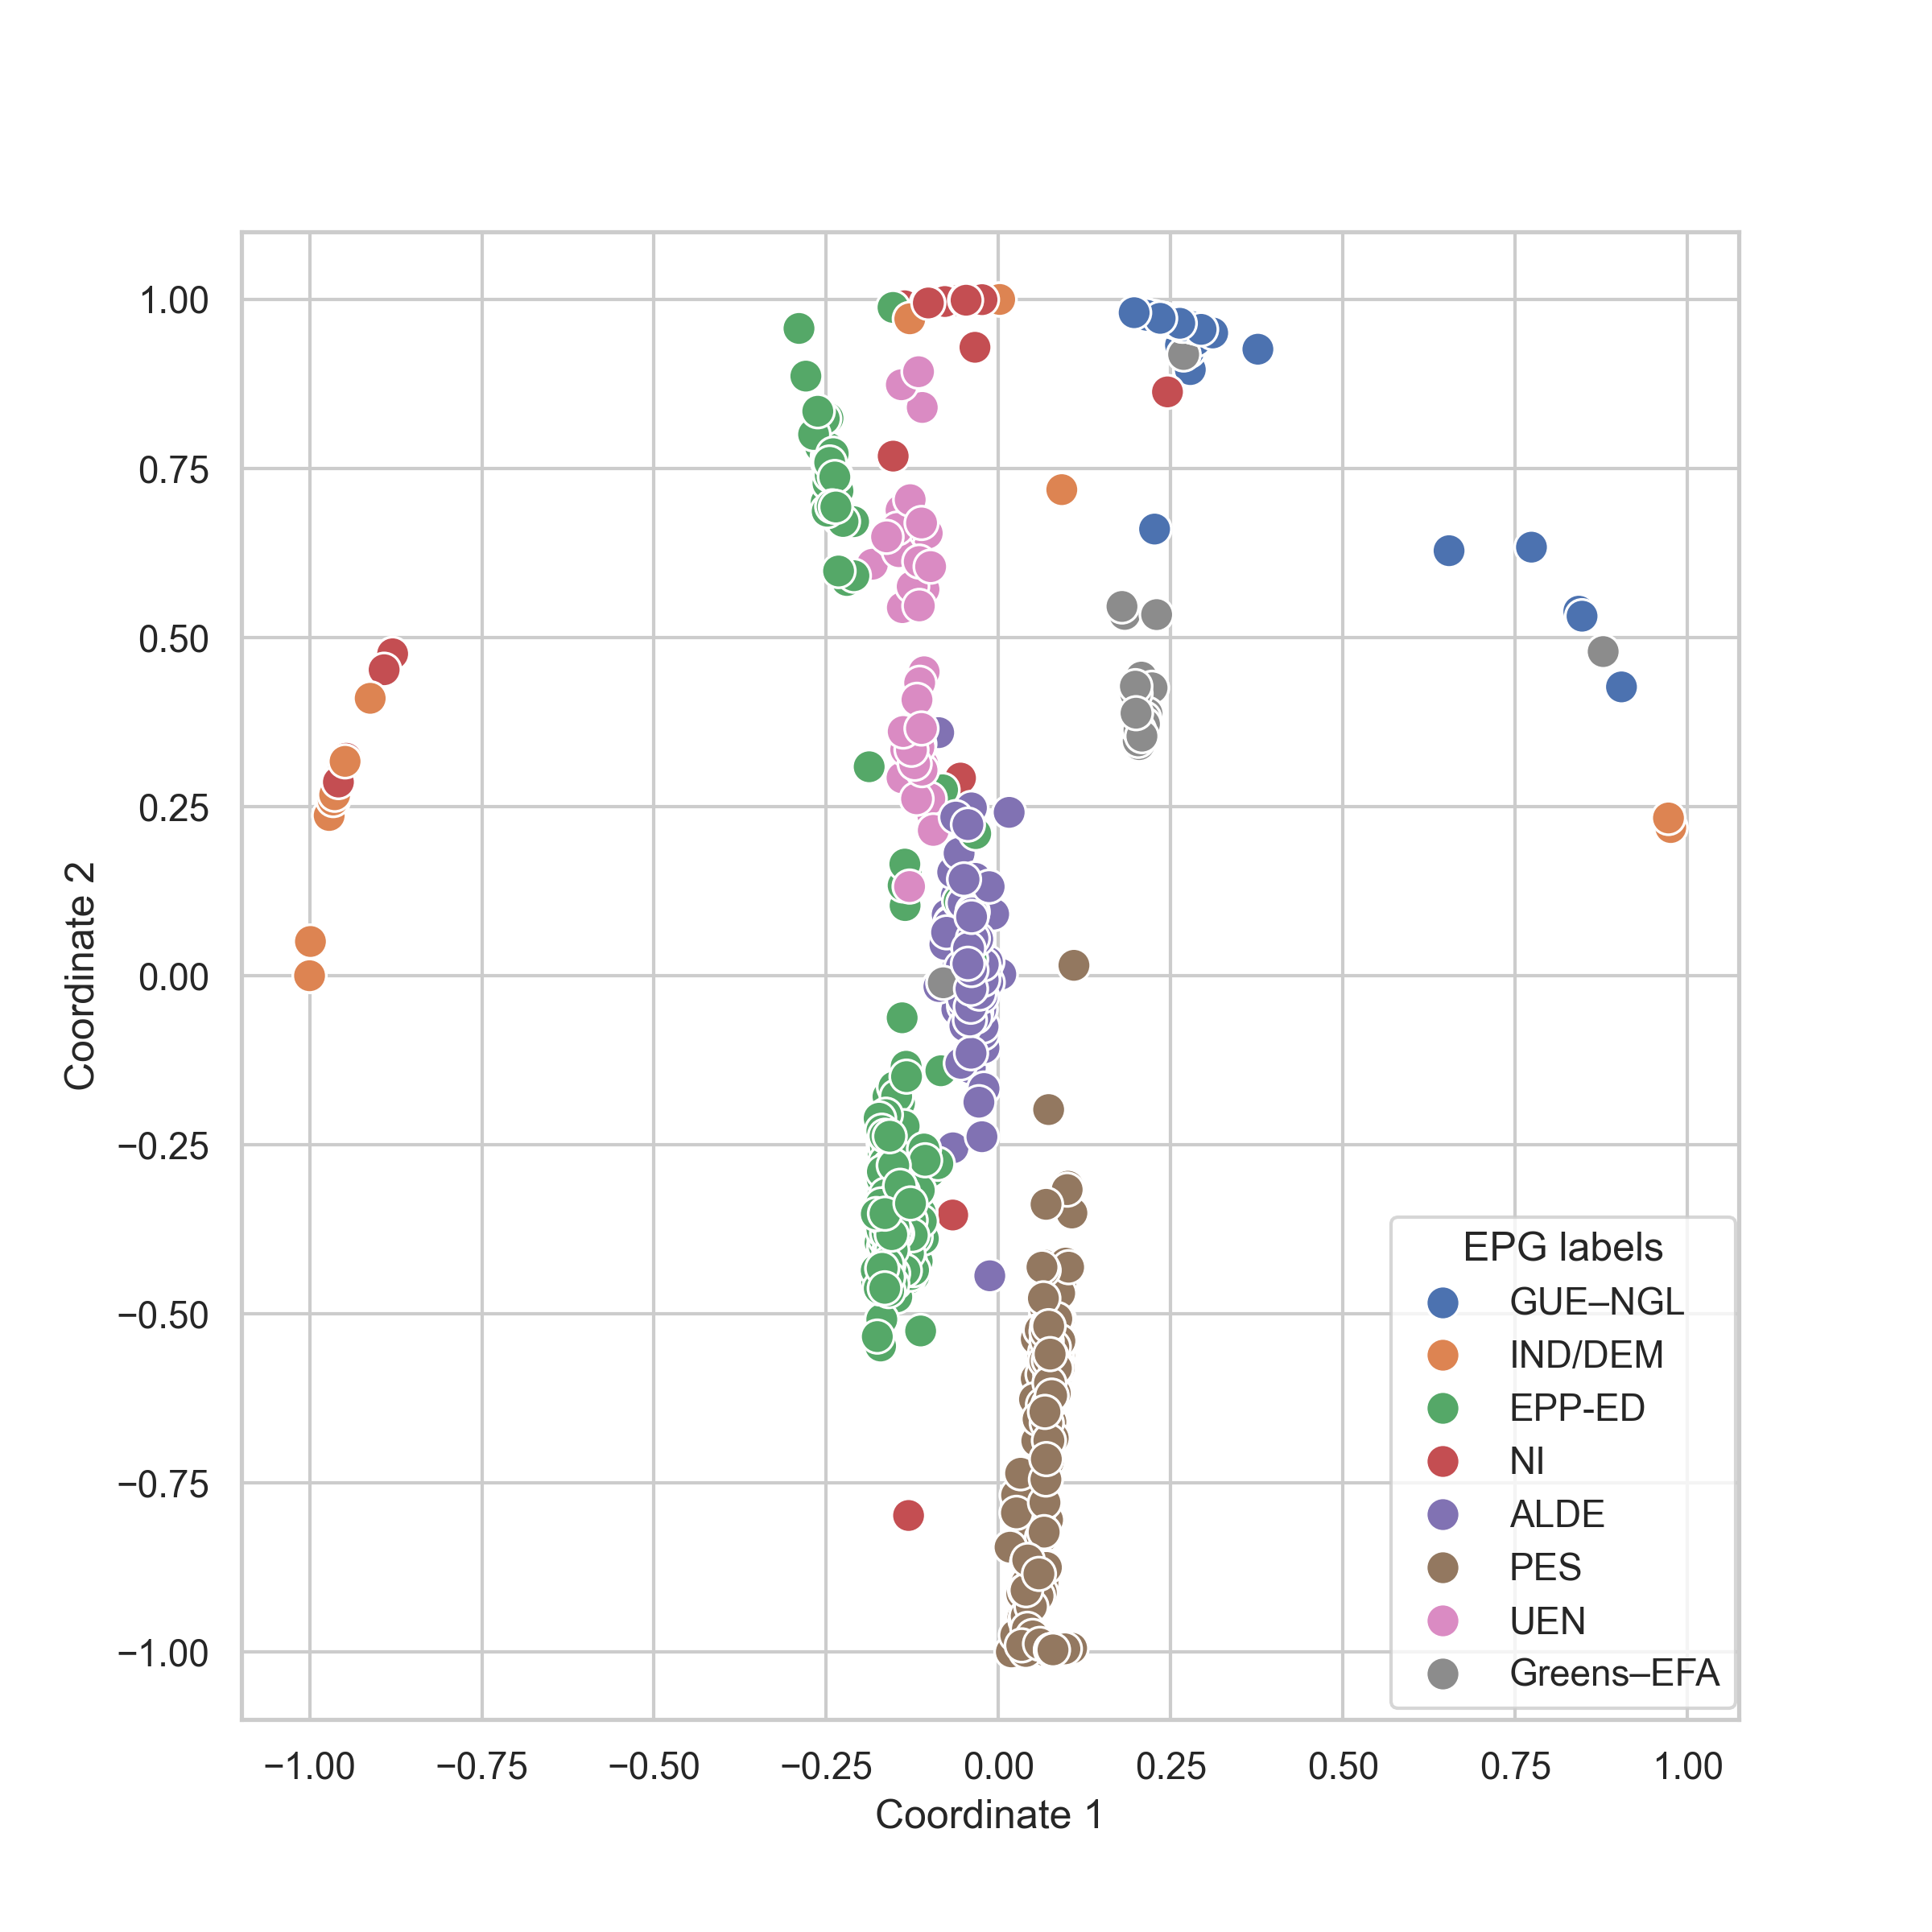
\includegraphics[width=1\textwidth]{Graphs/WNOMINATE2d.png}
                    \caption{Recreation of Ideal Points Analysis in European Parliament 6 using WNOMINATE}
                    \label{fig:WNOMINATE 6}
                \end{figure}



                \susbection{Comparison of results}
                In order to explicitly compare the results we achieved to the ones of Hix & Noury (2009) we would need
                to have
                access to the original coordinates produced by W-NOMINATE in their research. This data is
                unfortunately not available publicly, so the most feasible method of comparison is visual analysis
                of characteristics of both representations of ideal points. One can immediately notice that the
                positions of the main political groups in our map are inverted in relation to the map we are
                comparing with. This is likely due to a different MEP being chosen as the 'conservative' in the
                initialization of the algorithm. In order to compare the results more adequately, we decided to show
                a map with both dimensions inverted, to better match the original results.

                \begin{figure}[H]
                    \centering
                    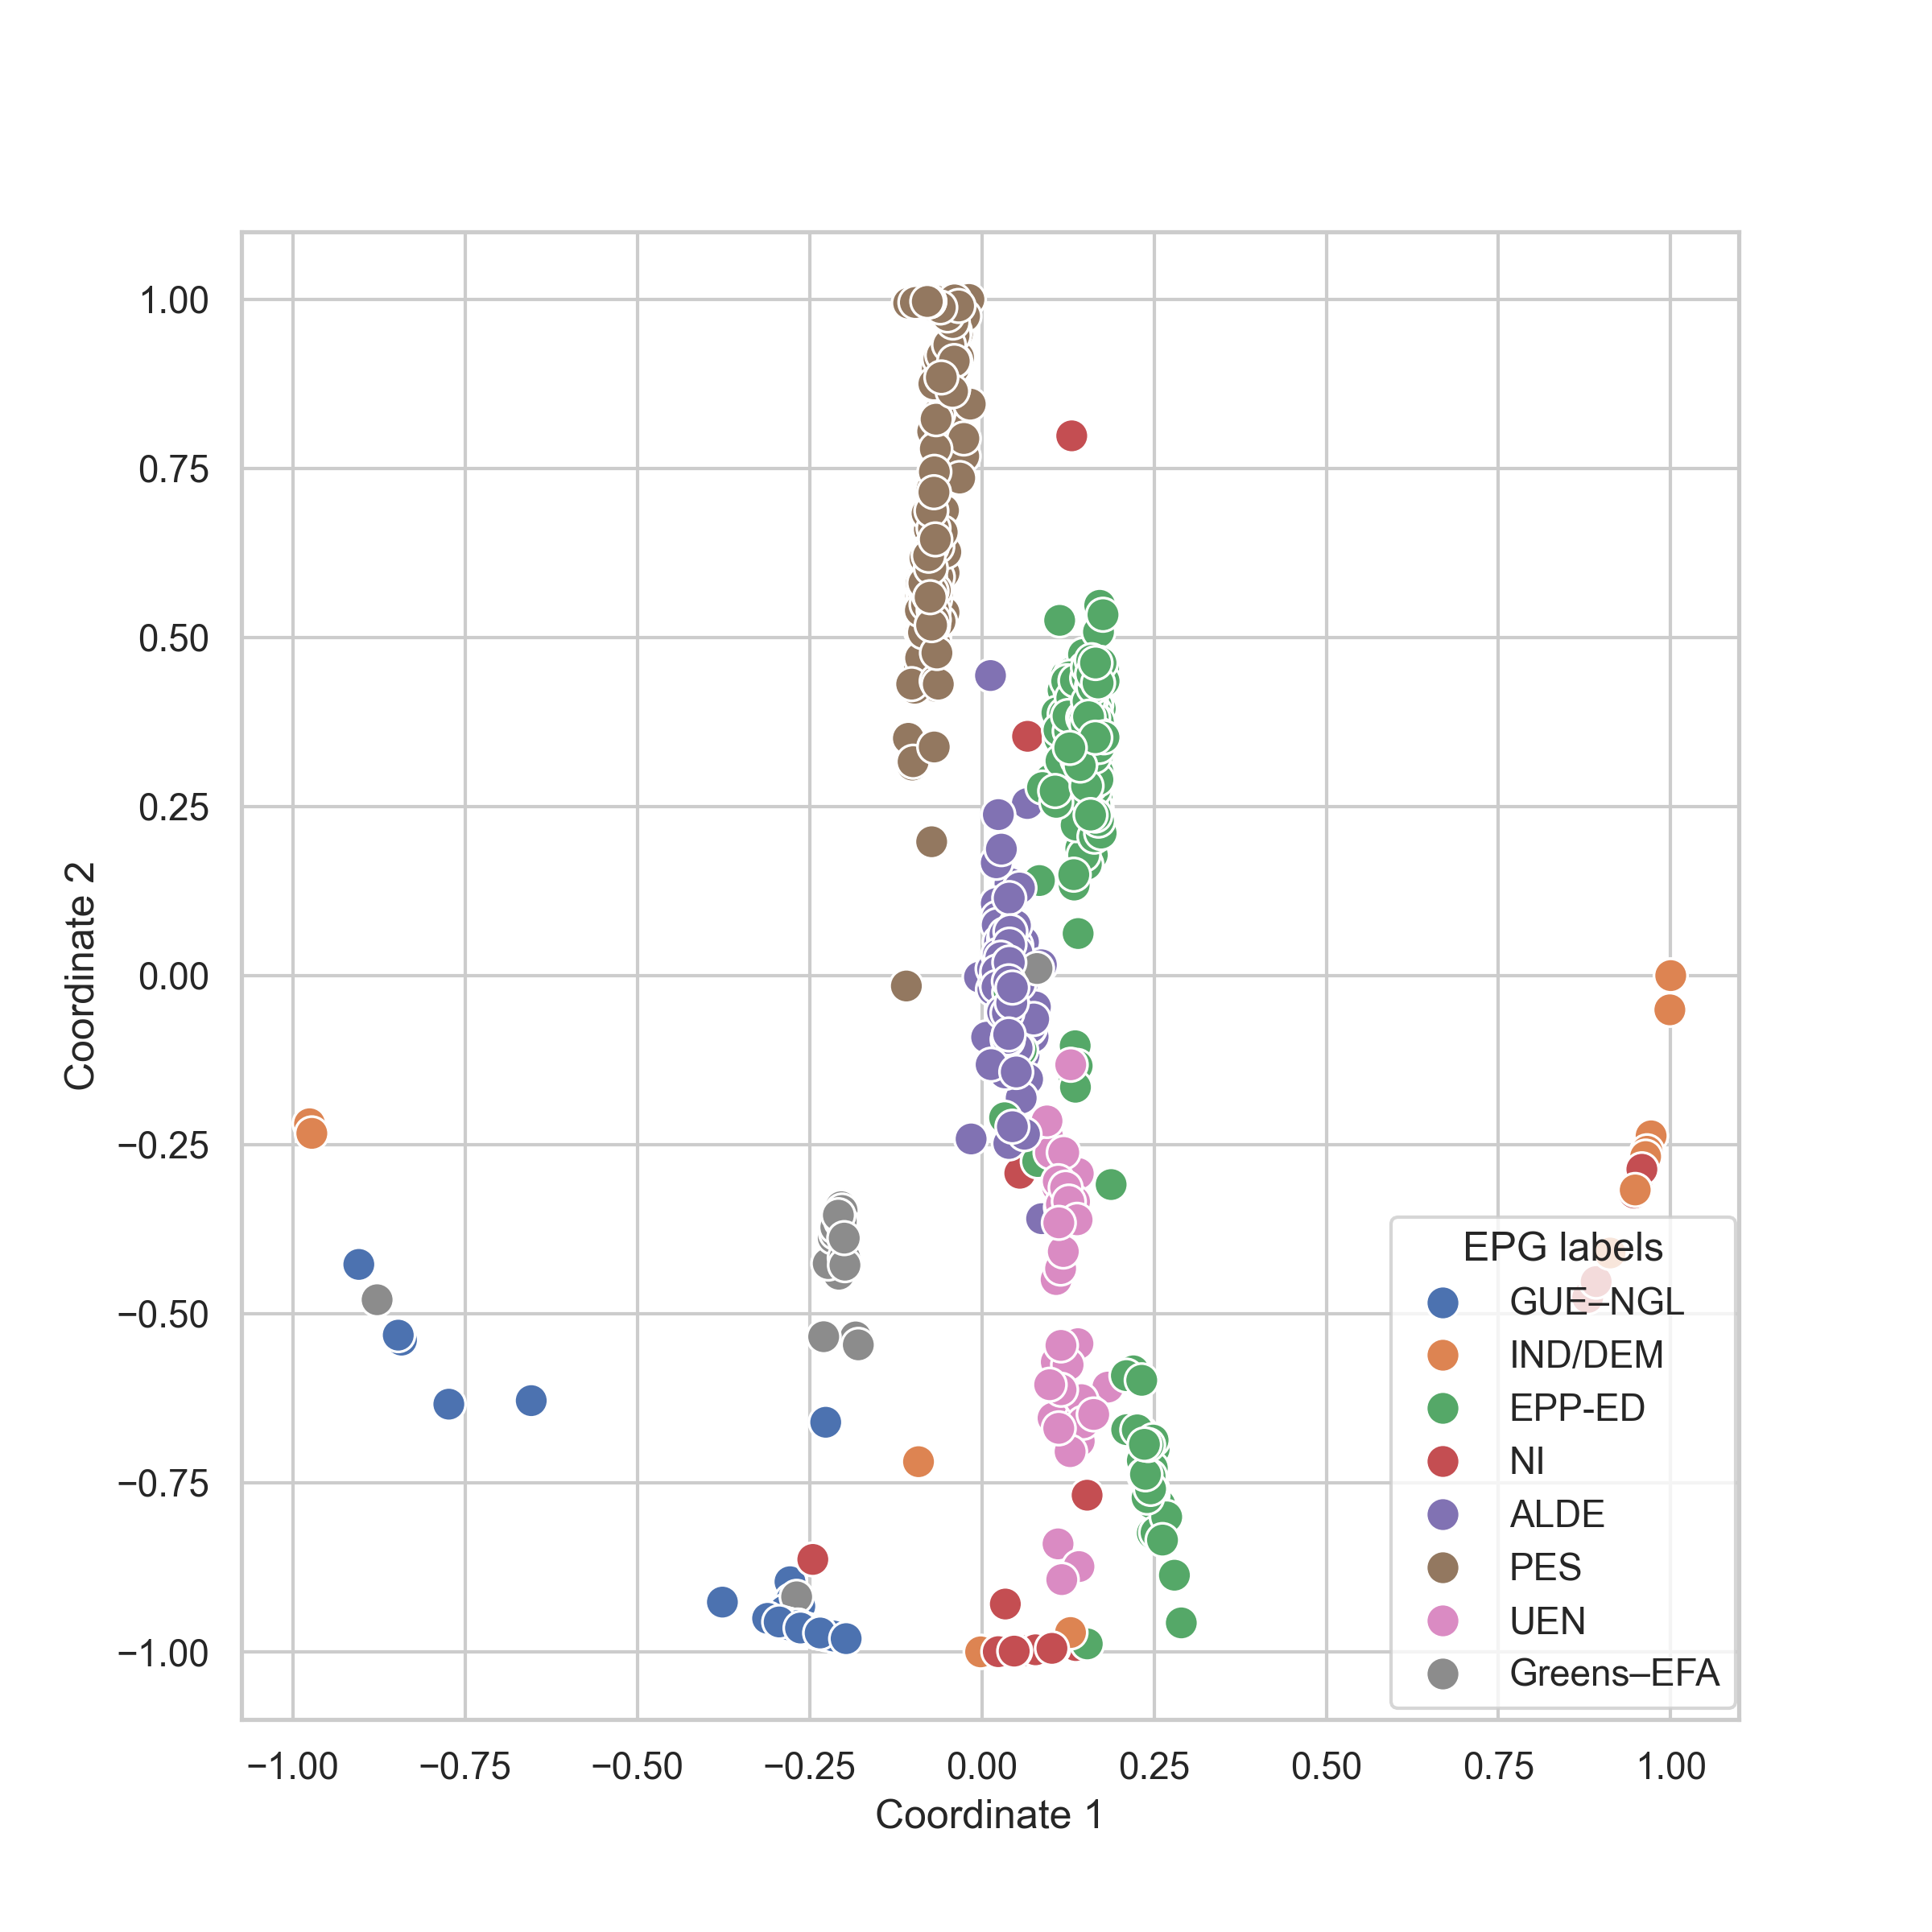
\includegraphics[width=1\textwidth]{Graphs/WNOMINATEflipped2d.png}
                    \caption
                    {Recreation of Ideal Points Analysis in European Parliament 6 using WNOMINATE with both dimensions
                    inverted}
                    \label{fig:WNOMINATE 6 FLIPPED}
                \end{figure}
                With maps aligned, several similar characteristics become apparent. The EPGs appear in similar
                clusters, with a similar alignment as in the original. The Socialists (PES in reproduction) are
                firmly in the range of
                -0.2 to 0 in the first dimension in both cases and 1 and 0.25 in the second dimension in the
                reproduction, but between 1 and 0.6 in the original work. The most likely explanation for this
                discrepancy is the polarity setting in the second dimension - if we chose a MEP that is closer to
                some of the
                Socialists in terms of ideal points than the one in Hix & Noury (2009) as a 'conservative' we would
                naturally
                bring the Socialists closer to the middle of the map, distorting the image. That seems to be the
                most competent explanation of this phenomenon. Again, however, we do not have a way of comparing the
                results directly and lack the knowledge of the 'conservative' used in the reproduced work.

                Similarly to the Socialists, other groups - such as Conservatives (EPP-ED), Liberals (ALDE),
                Nationalists (UEN) and Grens (Greens-EFA) are in comparable clusters to the previous research. The
                Radical Left (GUE-NGL), the Anti-Europeans (IND/DEM) and the Independents (NI) are located on
                opposite spectra of the map, along the borders of the unit sphere (an inherent feature of maps
                produced by W-NOMINATE are points with maximum distance of 1 from the center). This also reflects
                accurately the reproduced work.

                With such similar results, and without other means of confirming the similarity, we can plausibly
                establish a successful reproduction of the workflow that was used in Hix & Nouury (2009). This
                results allows us to conclude the integrity of the dataset and methods used.


        \section{Comparison of one-dimensional ideal points methods}
            As mentioned before, W-NOMINATE has some limitations - when computing ideal points with a greater number
            of datapoints, it takes
            Talk about computational limitations of WNOMINATE and how we can use emIRT to get similiar results.

            \subsection{emIRT}
                Talk about how to get the results, how to use the software etc etc. Show some preliminary graphs etc

            \subsection{WNOMINATE}
                Same stuff as before.

            \subsection{Comparison}
                Compare the results and show that they are basically the same, so we can use emIRT in base cases instead
                of WNOMINATE - and will do so in the future, with more bootstraps etc.


        \section{Initialization research}

            Establishing they are similar ish - we wanted to run emIRT with WNOMINATE starts and WNOMINATE with emIRT
            starts

            \subsection{Obtaining the starting values of WNOMIANTE}
                agreement matrix etc etc

            \subsection{Initializing emIRT with WNOMINATE starts}
                etc etc couldnt manage WNOMINATE to run

            \subsection{Comparing the results}
                comparing emIRT normal to not normal


        \section{High-dimensional ideal points}
            Running WNOMINATE for high d is hard etc etc

            \subsection{Obtaining the ideal points using WNOMINATE}
                what i had to do etc etc

            \subsection{Interpretation of dimensions}
                normal interpretations, what can you do maybe more, why more dimensions are usually not used so much etc
                etc


        \section{Principal Component Analysis}

            kinda to do
            \susbection{Obtaining ideal points estimates using PCA}

            \subsection{Comapring with starting points of WNOMINATE}

            \subsection{Using Procrustes Rotation for high-dimensional comparison}


    \chapter{Analysing the structure of missing data}


        \section{Overview of missing data}

            \subsection{Types of missing data in the dataset}

            \subsection{Describing the missingess}


        \section{Impact of ideology on missingness}

            \subsection{Model}

            \subsection{Results}


    \chapter{Conclusions}
\end{document}